\documentclass[11pt,a4paper]{article}

\usepackage{amsmath,amssymb,amsthm}
\usepackage{mathtools}
\usepackage{geometry}
\usepackage{hyperref}
\usepackage{xcolor}
\usepackage{tikz}
\usetikzlibrary{arrows.meta,positioning,decorations.markings,calc}
\usepackage{tcolorbox}
\tcbuselibrary{skins,breakable}
\usepackage{enumitem}
\usepackage{microtype}
\usepackage{booktabs}

\geometry{margin=2.3cm}
\hypersetup{colorlinks=true,linkcolor=blue!60!black,urlcolor=blue!60!black}

\definecolor{gunnaryellow}{RGB}{255,236,179}
\definecolor{gunnarpink}{RGB}{255,182,205}
\definecolor{gunnarblue}{RGB}{170,210,240}
\definecolor{commentboxbg}{RGB}{240,245,250}
\definecolor{exampleboxbg}{RGB}{246,250,238}

\newtcolorbox{commentbox}[1][]{
  colback=commentboxbg, colframe=blue!50!black,
  fonttitle=\bfseries, title=Commentary, breakable, #1
}
\newtcolorbox{examplebox}[1][]{
  colback=exampleboxbg, colframe=green!40!black,
  fonttitle=\bfseries, breakable, #1
}

\newcommand{\hl}[1]{\colorbox{gunnaryellow}{$#1$}}
\newcommand{\hpink}[1]{\colorbox{gunnarpink}{$#1$}}

\title{\vspace{-1.2cm}More messy diagrammatics --- the $n$-rail challenge\\[2pt]
{\large Reply to Gunnar's note of 7~May 2026}}
\author{Sirsh \& Claude}
\date{7 May 2026}

\begin{document}
\maketitle

\vspace{-1em}
\begin{commentbox}[title=One-line takeaway]
The $n$-rail count is the matrix element $\big(L^{m}\big)_{00}$ of the
\textbf{weighted graph Laplacian} $L=D-A$ on $K_n$ with edge weights $v_{ij}$.
For uniform coupling $v_{ij}\!\equiv\!v$ this collapses to
$\boxed{\;W^{(n)}_m = \tfrac{n-1}{n}\,(nv)^m\;}$ which extends your
$\tfrac12(2v_1)^m$ for $n{=}2$ to $\tfrac23(3v)^m,\;\tfrac34(4v)^m,\dots$\
The loop integrals factor cleanly off the combinatorics: each off-path rail
decomposes into a sequence of return-excursions, and each excursion is a
single one-loop kinematic kernel.
\end{commentbox}

%==================================================
\section{The challenge, restated}
%==================================================

You consider a theory with two rail-coupling vertices,
\[
\Gamma^{+}_{ij}\;=\;
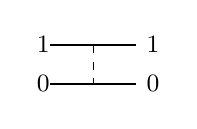
\begin{tikzpicture}[baseline=-0.6ex,scale=0.55]
  \draw[thick] (-1,0.45)--(1,0.45) node[right]{\small$1$};
  \node at (-1.15,0.45){\small$1$};
  \draw[thick] (-1,-0.45)--(1,-0.45) node[right]{\small$0$};
  \node at (-1.15,-0.45){\small$0$};
  \draw[dashed] (0,0.45)--(0,-0.45);
\end{tikzpicture}\;\;= +v_{ij},
\qquad
\Gamma^{-}_{ij}\;=\;
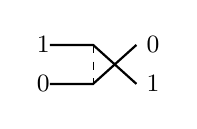
\begin{tikzpicture}[baseline=-0.6ex,scale=0.55]
  \draw[thick] (-1,0.45)--(0,0.45)--(1,-0.45) node[right]{\small$1$};
  \node at (-1.15,0.45){\small$1$};
  \draw[thick] (-1,-0.45)--(0,-0.45)--(1,0.45) node[right]{\small$0$};
  \node at (-1.15,-0.45){\small$0$};
  \draw[dashed] (0,0.45)--(0,-0.45);
\end{tikzpicture}\;\;= -v_{ij},
\]
with $v_{ij}=v_{ji}$ the symmetric coupling between rail $i$ and rail $j$, and
the propagator on every rail is $G(\omega)=(-i\omega+r)^{-1}$.

You restrict to \emph{$n$-rail diagrams with one rail of type $1$ (the
``$1$-rail''---initially rail $0$) and $n-1$ rails of type $0$}. By tracking
``the path the $1$ takes,'' you arrive at the local rule:
\begin{itemize}[leftmargin=2em,itemsep=1pt]
  \item every vertex where the $1$ \emph{stays} on its current rail and a
        bridge crosses to another rail $j$ contributes \hl{+v_{aj}};
  \item every vertex where the $1$ \emph{swaps} from rail $a$ to rail $b$
        contributes \hl{-v_{ab}}.
\end{itemize}
For $n=2$ the $m$-th-order weighted sum is \hl{\tfrac12(2v_1)^m}, and the open
question is

\begin{commentbox}[title=The two challenges]
\textbf{(C1)}\; Extend $\tfrac12(2v_1)^m$ to $n=3,4,\dots$ in closed form,
with the $v_{ij}$ kept symbolic (so that one can read off which couplings
contribute at which order).\\[2pt]
\textbf{(C2)}\; Account for the loop integrals (the analytic side --- not
just the symbol-level sign and weight) within the AC framework.
\end{commentbox}

%==================================================
\section{The combinatorial answer (C1): walks on the weighted complete graph}
%==================================================

\paragraph{The transfer step.}
Between two consecutive vertices on the $1$'s path, the $1$ sits on a single
rail $a$. At the next vertex it either
\begin{itemize}[leftmargin=2em,itemsep=1pt]
  \item \emph{stays} on rail $a$, with a bridge to some rail $j\neq a$, weight $+v_{aj}$;
  \item \emph{swaps} from rail $a$ to a chosen rail $b\neq a$, weight $-v_{ab}$.
\end{itemize}
Define the rail-to-rail transfer matrix $T$ with entries
\[
T_{aa}\;=\;\sum_{j\neq a}v_{aj}\quad(\text{stay, summed over bridge target}),
\qquad
T_{ab}\;=\;-v_{ab}\quad(a\neq b,\;\text{swap}).
\]
Read off the structure: $T_{aa}$ is the weighted degree of vertex $a$ in the
complete graph $K_n$ with edge weights $v_{ij}$, and $T_{ab}$ is the
\emph{negated} adjacency. Therefore
\begin{commentbox}[title=The transfer matrix is the graph Laplacian]
\[
\boxed{\;T \;=\; L \;=\; D-A,\qquad
D_{aa}=\!\!\sum_{j\neq a}\!v_{aj},\;\; A_{ab}=v_{ab}\,(1-\delta_{ab}).\;}
\]
\end{commentbox}
The whole sign-and-symmetry-factor accounting collapses into one line: the
$1$'s path is a length-$m$ walk on $\{0,1,\dots,n-1\}$ generated by $L$,
beginning and ending at rail $0$, so the order-$m$ weighted sum is
\[
\boxed{\;W^{(n)}_m \;=\; \big(L^{m}\big)_{00}.\;}
\]

\paragraph{Sanity check: $n=2$.}
With one coupling $v_{01}\equiv v$ and rails $\{0,1\}$,
\[
L \;=\; v\begin{pmatrix} \phantom{-}1 & -1 \\ -1 & \phantom{-}1\end{pmatrix},
\qquad
\text{eigenvalues}\;\;\{0,\,2v\},\quad
\text{eigenvectors}\;\;\tfrac{1}{\sqrt 2}(1,1),\;\tfrac{1}{\sqrt2}(1,-1).
\]
Then $L^m = (2v)^m\,P_{\!\perp}$ with $P_{\!\perp}=\tfrac12\!\begin{pmatrix}1&-1\\-1&1\end{pmatrix}$,
and $\big(L^m\big)_{00}=\tfrac12(2v)^m$ --- exactly your formula. \,\checkmark

\paragraph{General $n$, uniform coupling.}
If $v_{ij}\equiv v$, then $L=v(nI-J)$ where $J$ is the all-ones matrix.
The spectrum is $\{0,nv,nv,\dots,nv\}$ (multiplicity $n-1$ on the
$\mathbf 1^{\perp}$ subspace), so
\[
L^{m} \;=\; (nv)^{m}\,P_{\!\perp},\qquad P_{\!\perp}=I-\tfrac{1}{n}J,
\]
and the boundary matrix element is
\begin{equation}\label{eq:closed}
\boxed{\;
W^{(n)}_m \;=\; \big(L^m\big)_{00}\;=\;\frac{n-1}{n}\,(nv)^m.\;}
\end{equation}
This is the requested extension. The first values are
\[
\renewcommand{\arraystretch}{1.15}
\begin{array}{c|c|c|c|c}
n & 2 & 3 & 4 & 5\\\hline
W^{(n)}_m & \tfrac12(2v)^m & \tfrac23(3v)^m & \tfrac34(4v)^m & \tfrac45(5v)^m
\end{array}
\]
The pattern is intuitive: at order $m$ there are $n^{m}$ raw step sequences
(at each of $m$ vertices the $1$ chooses one of $n-1$ partner rails, with two
moves per partner --- stay or swap, signed); the projection onto walks
returning to rail $0$ extracts the $\frac{n-1}{n}$ Frobenius factor.

\paragraph{General $n$, distinct $v_{ij}$.}
Without uniformity the answer is the spectral expansion (for $m\!\geq\!1$)
\begin{equation}\label{eq:spectral}
W^{(n)}_m \;=\; \sum_{\alpha=1}^{n-1}\lambda_\alpha^{\,m}\,|\psi_\alpha(0)|^{2},
\end{equation}
with $L\psi_\alpha=\lambda_\alpha\psi_\alpha$ orthonormal and $\lambda_0=0$
dropping out for any $m\!\geq\!1$ (the constant eigenvector $\psi_0\propto\mathbf 1$
sits in the kernel of $L$). For the symbolic $v_{ij}$, this is
\[
W^{(n)}_m \;=\; \mathbf{e}_0^{\top}\,L^{m}\,\mathbf{e}_0,
\qquad L_{ij} \;=\; \delta_{ij}\!\sum_{k\neq i}v_{ik}\;-\;(1-\delta_{ij})\,v_{ij}.
\]
For example at $n=3$ in the basis $\{0,1,2\}$,
\[
L \;=\; \begin{pmatrix}
v_{01}+v_{02} & -v_{01} & -v_{02}\\
-v_{01} & v_{01}+v_{12} & -v_{12}\\
-v_{02} & -v_{12} & v_{02}+v_{12}
\end{pmatrix},
\]
and $\big(L^2\big)_{00} = (v_{01}+v_{02})^{2}+v_{01}^{2}+v_{02}^{2}$,
$\big(L^3\big)_{00} = (v_{01}+v_{02})^{3}+v_{01}^{2}(v_{01}+v_{02})
+v_{02}^{2}(v_{01}+v_{02})+v_{01}^{2}(v_{01}+v_{12})
+v_{02}^{2}(v_{02}+v_{12})+2v_{01}v_{02}v_{12}$, which one can
read term-by-term as the path enumeration on the rail graph
(``stay-stay'', ``stay-swap-swap'', etc.).

\paragraph{Connection to the bidegree-(1,1) Q1 result.}
This is the $n$-rail generalisation of the $n{=}2$ ladder result we sent on
29~Apr: there, projecting the four-variable vertex polynomial $\widehat V$
onto the bidegree-(1,1) sector gave
$\widehat T(z,w)=(z_1-z_2)(w_1-w_2)$, eigenvalue $\lambda{=}2$, and
$\langle b\,|\,\widehat T^{n}\,|\,b\rangle = 2^{n}$. The Laplacian above is
exactly that boundary-projected operator written in rail-state basis: the
antisymmetric mode of $K_2$ \emph{is} the $\mathbf 1^{\perp}$ eigenspace of
$L$. For $n\!\geq\!3$ the antisymmetric/symmetric language disappears and we
need the full Laplacian spectrum --- but the AC bookkeeping is identical.

%==================================================
\section{The analytic answer (C2): loop integrals attach as kinematic atoms}
%==================================================

The combinatorial sum \eqref{eq:closed}--\eqref{eq:spectral} only counts
\emph{symbol-level} weights. The analytic value of one diagram --- the
loop integrals over internal frequencies / momenta --- is built on top
of that count. The key observation is that for a fixed rail-walk $w$,
the diagram value factorises into two independent pieces:
\begin{commentbox}[title=The recipe for one diagram]
\[
\boxed{\;\Gamma(w) \;=\; \underbrace{S(w)}_{\text{symbol weight}}
\;\times\;\underbrace{K(w)}_{\text{kinematic kernel}}\;}
\]
where $S(w)$ is a product of vertex weights $\pm v_{ij}$ (no integrals)
and $K(w)$ is a product of propagator chains and loop integrals (no
$v_{ij}$). They never mix.
\end{commentbox}
The full $m$-th order contribution to the impurity self-energy is then
$\Gamma^{(m)} = \sum_{w}S(w)K(w)$ summed over all length-$m$ walks
$0\!\to\!0$. The Laplacian formula $\sum_{w}S(w) = (L^{m})_{00}$ from
\S\,2 collects the symbol part; what is left is to write down $K(w)$.

\subsection*{Step 1: how to read off the symbol weight $S(w)$}

A walk $w = (\text{vertex}_{1},\text{vertex}_{2},\dots,\text{vertex}_{m})$
is a sequence of $m$ moves, each one labelled by either ``stay'' or
``swap'' and the rail $j$ involved. The recipe is local --- one factor
per vertex --- and just transcribes Gunnar's local rule:
\begin{equation}\label{eq:symbol-weight}
S(w) \;=\; \prod_{t=1}^{m}\sigma_{t}\,v_{a_{t}j_{t}},
\qquad
\sigma_{t} = \begin{cases}+1 &\text{if vertex $t$ is a stay}\\
-1 &\text{if vertex $t$ is a swap}\end{cases},
\end{equation}
where $a_{t}$ is the rail the $1$ sits on just before vertex $t$ and
$j_{t}$ is the partner rail at that vertex. \emph{Example:} the walk
``stay-bridge-to-1, swap-onto-2, swap-back-to-0'' on rails $\{0,1,2\}$
gives $S = (+v_{01})(-v_{02})(-v_{02}) = +v_{01}v_{02}^{2}$.
This is just the product Gunnar wrote down; nothing analytic happens
here.

\subsection*{Step 2: how to compute the kinematic kernel $K(w)$}

The kernel is built from the propagator structure of the diagram. Two
ingredients, in order:

\paragraph{(a) The on-path piece (chain on the $1$'s worldline).}
Read the $1$'s worldline left-to-right. Between consecutive vertices
the $1$ sits on some rail and carries the external frequency $\omega$,
contributing one propagator $G(\omega) = (-i\omega+r)^{-1}$. With $m$
vertices there are $m{+}1$ such segments, so
\begin{equation}\label{eq:on-path}
K_{\text{on-path}}(w) \;=\; \prod_{\text{segments}}G(\omega)
\;=\; \frac{1}{(-i\omega+r)^{m+1}}.
\end{equation}
This factor is the same for every walk of length $m$ --- it does not
care about chunk pattern --- and is just the propagator dressing of the
external $1$-line.

\paragraph{(b) The off-path piece (one loop per visited bath rail).}
Now consider each bath rail $j$ \emph{separately}. Count how many
``stay-with-bridge-to-$j$'' vertices appear in $w$; call this number
$p_{j}(w)$. Then rail $j$ has $p_{j}$ insertions and (because it has
no external sources) closes into a single \textbf{$p_{j}$-cycle loop
integral}:
\begin{equation}\label{eq:off-path}
K_{j}(p_{j}) \;:=\;
\int\!\frac{d\omega'}{2\pi}\;\prod_{k=1}^{p_{j}}
G_{j}\!\big(\omega' - \Omega^{(j)}_{k}\big),
\end{equation}
where the $\Omega^{(j)}_{k}$ are external-frequency injections at the
$j$-rail vertices (determined by where in the walk the rail-$j$ visits
happen). The full kernel is then
\begin{equation}\label{eq:total-kernel}
K(w) \;=\; K_{\text{on-path}}(w)\;\cdot\;\prod_{j\,:\,p_{j}\geq 1}
K_{j}(p_{j}).
\end{equation}
The standard names of the $K_{j}(p_{j})$ are familiar:
\[
\renewcommand{\arraystretch}{1.2}
\begin{array}{c|l|l}
p_{j} & \text{name} & K_{j}(p_{j}) \\ \hline
1 & \text{tadpole} & \int\!d\omega'\,G_{j}(\omega') \\
2 & \text{bubble} & \int\!d\omega'\,G_{j}(\omega')G_{j}(\omega'{-}\Omega) \\
3 & \text{sunset (2-loop)} & \int\!d\omega'_{1}\,d\omega'_{2}\;G_{j}\,G_{j}\,G_{j} \\
p & (p{-}1)\text{-loop }p\text{-cycle} &
\int\prod_{k}G_{j}\big(\omega'-\Omega_{k}\big)
\end{array}
\]
Swap vertices do \emph{not} contribute insertions on bath rails ---
they live on the $1$'s worldline (they change which rail the $1$ is
sitting on, no extra bath-rail visit). So $p_{j}$ counts only stays
with bridge-to-$j$.

\paragraph{Why the kernel depends only on the chunk pattern.}
Two walks with the same chunk pattern (same sequence of run-lengths of
the $1$ on a single rail) have the same multiset $\{p_{j}\}$ of
off-path insertion counts, up to relabelling of bath rails. They
therefore share $K(w)$. This is why \emph{two distinct walks can carry
the same kernel} --- and why the $K$-library is much smaller than the
walk count.

\paragraph{Worked examples (a small atlas).}
Four canonical low-order diagrams illustrate how the recipe
(Steps 1--2 above) attaches each rail-walk to an explicit
$S(w)\!\cdot\!K(w)$ value. Solid lines are propagators (arrow on
the $1$-rail to mark the impurity worldline), dashed verticals are
4-point vertices with the indicated $\pm v_{ij}$ weight, and a closing
arc on a bath rail indicates the rail closing into a loop. Each box
states $S(w)$ from \eqref{eq:symbol-weight}, the per-rail insertion
counts $\{p_{j}\}$, and $K(w)$ from
\eqref{eq:on-path}--\eqref{eq:total-kernel}.

\medskip
\textit{(i) Order $m{=}1$, stay-vertex with bridge $0\!\to\!j$.}
The $1$ stays on rail $0$; rail $j$ is visited once and closes into a
tadpole.
\begin{center}
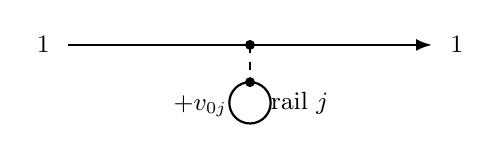
\begin{tikzpicture}[scale=1.05]
  \draw[thick,-{Latex[length=2mm]}] (-2.2,0.5)--(2.2,0.5);
  \node at (-2.5,0.5) {\small$1$}; \node at (2.5,0.5) {\small$1$};
  \filldraw (0,0.5) circle (1.5pt);
  \draw[dashed] (0,0.5)--(0,0.05);
  \filldraw (0,0.05) circle (1.5pt);
  \draw[thick] (0,-0.20) circle (0.25);
  \node at (0.6,-0.20) {\small rail $j$};
  \node[anchor=north] at (-0.6,0.0) {\small$+v_{0j}$};
\end{tikzpicture}
\end{center}
\textit{Apply the recipe.}
\;Step 1: one stay vertex, $\sigma_{1}{=}+1$, partner rail $j$
$\Rightarrow S = +v_{0j}$.
\;Step 2: $p_{j}{=}1$ (single bridge to $j$), so $K_{j}=\mathcal T$
(tadpole), and the on-path chain has $m{+}1{=}2$ propagators:
\[
S = +v_{0j},\qquad
K \;=\; \frac{1}{(-i\omega+r)^{2}}\,\cdot\,
\underbrace{\int\!\frac{d\omega'}{2\pi}\,\frac{1}{-i\omega'+r}}_{\mathcal T(r)}.
\]
Chunk pattern: $(2)$ on rail $0$. The tadpole is absorbed into
mass renormalisation in any sensible scheme.

\medskip
\textit{(ii) Order $m{=}2$, two stays both bridging to the same rail $j$.}
Rail $j$ is visited at two consecutive insertions; the segment between
them closes into a bubble.
\begin{center}
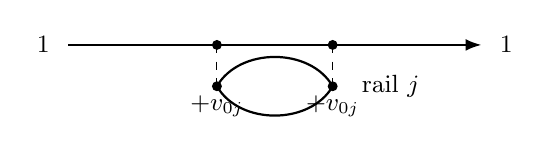
\begin{tikzpicture}[scale=1.05]
  \draw[thick,-{Latex[length=2mm]}] (-2.5,0.5)--(2.5,0.5);
  \node at (-2.8,0.5) {\small$1$}; \node at (2.8,0.5) {\small$1$};
  \filldraw (-0.7,0.5) circle (1.5pt);
  \filldraw ( 0.7,0.5) circle (1.5pt);
  \draw[dashed] (-0.7,0.5)--(-0.7,0.0);
  \draw[dashed] ( 0.7,0.5)--( 0.7,0.0);
  \filldraw (-0.7,0.0) circle (1.5pt);
  \filldraw ( 0.7,0.0) circle (1.5pt);
  \draw[thick] (-0.7,0.0) to[bend right=60] (0.7,0.0);
  \draw[thick] (-0.7,0.0) to[bend left=60]  (0.7,0.0);
  \node at (1.4,0.0) {\small rail $j$};
  \node[anchor=north] at (-0.7,0.0) {\small$+v_{0j}$};
  \node[anchor=north] at ( 0.7,0.0) {\small$+v_{0j}$};
\end{tikzpicture}
\end{center}
\textit{Apply the recipe.}
\;Step 1: two stay vertices, both with partner rail $j$
$\Rightarrow S = (+v_{0j})(+v_{0j}) = v_{0j}^{2}$.
\;Step 2: $p_{j}{=}2$ insertions $\Rightarrow K_{j}=\mathcal B$ (bubble),
on-path chain $1/(-i\omega+r)^{3}$:
\[
S = v_{0j}^{2},\qquad
K \;=\; \frac{1}{(-i\omega+r)^{3}}\,\cdot\,
\underbrace{\int\!\frac{d\omega'}{2\pi}\,
G_{j}(\omega')\,G_{j}(\omega'{-}\Omega)}_{\mathcal B(\Omega;r)}.
\]
Chunk pattern: $(3)$ on rail $0$. The bubble's external $\Omega$ is the
frequency flowing through the $1$ between the two vertices.

\medskip
\textit{(iii) Order $m{=}2$, swap-and-return $0\!\to\!j\!\to\!0$.}
The $1$ swaps onto rail $j$ at the first vertex and back at the second.
There is \emph{no closed loop}: the rail-$j$ segment between the swaps is
part of the $1$'s worldline, not a bath excursion.
\begin{center}
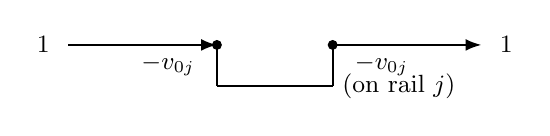
\begin{tikzpicture}[scale=1.05]
  \draw[thick,-{Latex[length=2mm]}] (-2.5,0.5)--(-0.7,0.5);
  \draw[thick] (-0.7,0.5)--(-0.7,0.0);
  \draw[thick] (-0.7,0.0)--(0.7,0.0);
  \draw[thick] (0.7,0.0)--(0.7,0.5);
  \draw[thick,-{Latex[length=2mm]}] (0.7,0.5)--(2.5,0.5);
  \node at (-2.8,0.5) {\small$1$}; \node at (2.8,0.5) {\small$1$};
  \filldraw (-0.7,0.5) circle (1.5pt);
  \filldraw ( 0.7,0.5) circle (1.5pt);
  \node at (1.5,0.0) {\small (on rail $j$)};
  \node[anchor=east] at (-0.85,0.25) {\small$-v_{0j}$};
  \node[anchor=west] at ( 0.85,0.25) {\small$-v_{0j}$};
\end{tikzpicture}
\end{center}
\textit{Apply the recipe.}
\;Step 1: two swap vertices $\Rightarrow S = (-v_{0j})(-v_{0j}) = +v_{0j}^{2}$.
\;Step 2: \emph{no} stay-vertex bridges, so $p_{j}{=}0$ for every bath
rail --- \textbf{no loop integrals at all}. The whole kernel is just the
on-path chain (now passing through three rail-segments: $0\!\to\!j\!\to\!0$):
\[
S = +v_{0j}^{2},\qquad
K \;=\; \frac{1}{(-i\omega+r)^{3}}\quad\text{(chain only, no $\int d\omega'$)}.
\]
Chunk pattern: $(1,1,1)$ --- one segment on rail $0$, one on rail $j$,
one back on rail $0$. \textbf{Compare with (ii):} same symbol weight
$+v_{0j}^{2}$, completely different kernel. The Laplacian
$\big(L^{2}\big)_{00}$ collects both into the $2v_{0j}^{2}$ coefficient
at the symbol level; the recipe keeps them distinct on the analytic
side. This is the cleanest demonstration that $S$ and $K$ are
independent factors.

\medskip
\textit{(iv) Order $m{=}3$, three stays bridging to the same rail $j$.}
Rail $j$ has three consecutive insertions; the $j$-segments form a closed
$3$-cycle = sunset (2-loop).
\begin{center}
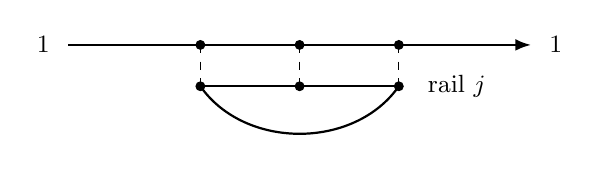
\begin{tikzpicture}[scale=1.05]
  \draw[thick,-{Latex[length=2mm]}] (-2.8,0.5)--(2.8,0.5);
  \node at (-3.1,0.5) {\small$1$}; \node at (3.1,0.5) {\small$1$};
  \filldraw (-1.2,0.5) circle (1.5pt);
  \filldraw ( 0.0,0.5) circle (1.5pt);
  \filldraw ( 1.2,0.5) circle (1.5pt);
  \draw[dashed] (-1.2,0.5)--(-1.2,0.0);
  \draw[dashed] ( 0.0,0.5)--( 0.0,0.0);
  \draw[dashed] ( 1.2,0.5)--( 1.2,0.0);
  \filldraw (-1.2,0.0) circle (1.5pt);
  \filldraw ( 0.0,0.0) circle (1.5pt);
  \filldraw ( 1.2,0.0) circle (1.5pt);
  \draw[thick] (-1.2,0.0)--(0.0,0.0);
  \draw[thick] ( 0.0,0.0)--(1.2,0.0);
  \draw[thick] (-1.2,0.0) to[bend right=55] (1.2,0.0);
  \node at (1.9,0.0) {\small rail $j$};
\end{tikzpicture}
\end{center}
\textit{Apply the recipe.}
\;Step 1: three stays, all to rail $j$
$\Rightarrow S = (+v_{0j})^{3}$.
\;Step 2: $p_{j}{=}3 \Rightarrow K_{j}=\mathcal S$ (sunset, 2-loop):
\begin{align*}
S \;&=\; v_{0j}^{3},\\
K \;&=\; \frac{1}{(-i\omega+r)^{4}}\,\cdot\,
\underbrace{\int\!\frac{d\omega'_{1}\,d\omega'_{2}}{(2\pi)^{2}}\;
G_{j}(\omega'_{1})\,G_{j}(\omega'_{2})\,G_{j}(\omega'_{1}{+}\omega'_{2}{-}\Omega_{12})}_{\mathcal S(\Omega_{1},\Omega_{2};r)}.
\end{align*}
Chunk pattern: $(4)$ on rail $0$. Standard 2-loop sunset.

\medskip
At higher order $m$, partitions of $m{+}1$ index the kernel library:
$(m{+}1)\!\to\!$\,closed cycle on one bath rail (single-rail $m$-loop),
$(m,1)\!\to\!$\,closed cycle plus tadpole, etc. Cases (ii)--(iv) sit in
the all-bridges sub-class; case (iii) is representative of the
swap-induced no-loop pieces. The rest of the chunk-pattern library
combines these.

\paragraph{Why the kernels are bounded in number.}
This is the \emph{rein-in} you asked about: even though the number of full
diagrams grows like $(nv)^{m}$, the number of \emph{distinct kinematic
kernels} is bounded by the partition number $p(m{+}1)$
($\!=\!1,2,3,5,7,11,15,22,\dots$): two walks with different rail labels but
the same chunk-length pattern (the partition of $m{+}1$ into the consecutive
runs of the $1$ on a single rail) share their kernel. The actual count is
generically below $p(m{+}1)$ because not every partition is realised at a
given $n$; e.g.\ at $n{=}3,\,m{=}5$ direct enumeration gives $8$ distinct
chunk-patterns (verified in \texttt{poc\_laplacian.py}), all $342$ raw
trajectories collapse onto these $8$ master integrals weighted by Laplacian
path multiplicities. \emph{This} is what AC buys you on the analytic side: a
contraction from $(\text{many walks})\;\to\;(\text{a finite kernel library})$.

\paragraph{Where the AC lens actually kicks in (and where it does not).}
The recipe in Steps 1--2 is just Gunnar's local rule transcribed
diagram-by-diagram --- there is no AC \emph{magic} in it. The AC lens
enters when we trade the per-diagram view for the
\textbf{generating function view}: package the entire perturbation series
into one object and let its analytic properties answer questions about
the whole series at once.

\smallskip
Concretely, define
\[
\mathcal G^{(n)}(z;\{v_{ij}\}) \;:=\; \sum_{m\geq 0} W^{(n)}_{m}\, z^{m}
\;=\; \big[(I - zL)^{-1}\big]_{00},
\]
which packages the symbol-side (Laplacian path weights) at all orders.
Many questions which \emph{look} like ``please compute and tabulate
$10^{6}$ diagrams'' become one-line readings off
$\mathcal G^{(n)}(z;\cdot)$:

\begin{commentbox}[title=Translation table: per-diagram question $\;\Longleftrightarrow\;$ AC reading]
\renewcommand{\arraystretch}{1.1}
\begin{tabular}{p{0.40\linewidth}p{0.55\linewidth}}
\toprule
\textbf{Per-diagram question} & \textbf{AC reading on $\mathcal G$} \\
\midrule
``At what rate does $W^{(n)}_{m}$ grow as $m\!\to\!\infty$?'' &
Dominant pole of $\mathcal G$ at $z=\lambda_{1}^{-1}$ (F-S Thm.~V.7);
for uniform $v$, $\lambda_{1}=nv$. \\
``What is the exact prefactor of $(nv)^{m}$?'' &
Residue of $\mathcal G$ at the dominant pole; for uniform $v$,
$\tfrac{n-1}{n}$ from the numerator zero $1{-}zv$. \\
``Order-$m$ split by channel $0$--$1$ usage?'' &
Mark $v_{01}\!\to\!v_{01}u$; coefficient of $u^{k}$ counts walks with
exactly $k$ uses of $v_{01}$ (\S\,4 (3)). \\
``Forbid one channel: new growth?'' &
Set $v_{ij}{=}0$ in $\mathcal G$; new dominant pole gives the
restricted rate (\S\,4 (3)). \\
``All-orders foreground given background integrated out?'' &
Schur reduce $\mathcal G$: one rational function with
frequency-dependent self-energy $\Sigma(z)$ (\S\,4 (4)). \\
``Truncate to short off-rail propagation?'' &
Matrix continued fraction obtained by recursive Schur peel; depth-$k$
truncation keeps $\leq k$ powers of the off-rail block (\S\,4 (5)).
Used as a structural device; the precise walk-counting interpretation
depends on the truncation convention. \\
\bottomrule
\end{tabular}
\end{commentbox}

\smallskip
\textbf{The point:} the rules of the diagram game are local (one factor
per vertex), but \emph{global} questions about the perturbation series
become poles, residues, zeros, and rational-function manipulations of
$\mathcal G$. The AC lens is precisely the dictionary between the two.
\S\,4 develops it into a working toolkit; the one-line takeaway is that
\emph{any time you need to know something about ``all the diagrams''
without computing them, the right object to manipulate is}
$\mathcal G^{(n)}(z;\{v_{ij}\})$.

\smallskip
What the AC lens \emph{does not} buy you is the explicit kinematic
kernel for an individual chunk pattern --- those tadpole / bubble /
sunset integrals are still genuine analytic work; AC reduces \emph{how
many distinct ones you need} (the $p(m{+}1)$ bound), not the difficulty
of any single one.

\paragraph{Reading off the symmetry factor of each kernel.}
A natural follow-up: \emph{can we read off the multiplicity / symmetry
factor of each kernel from the AC machinery?} Yes, in closed form. For
an unordered chunk-length partition
$\boldsymbol\lambda=(\ell_1,\dots,\ell_k)$ of $m{+}1$ with $c_p$ parts
of length $p$, the signed multiplicity of the kernel labelled by
$\boldsymbol\lambda$ at uniform coupling on $K_n$ factorises into four
combinatorial pieces, each derivable from the GF:
\begin{equation}\label{eq:multiplicity}
\boxed{\;
\mu_{\boldsymbol\lambda}^{(n)}(m)
\;=\;
\underbrace{\frac{k!}{\prod_{p\geq 1}c_p!}}_{\text{time-ordering}}
\;\times\;
\underbrace{A_{00}^{\,k-1}(K_n)}_{\text{rail-labeling}}
\;\times\;
\underbrace{(n-1)^{m+1-k}}_{\text{stays}}
\;\times\;
\underbrace{(-1)^{k-1}}_{\text{swap sign}}
\;}
\end{equation}
where $A=J_n-I_n$ is the no-self-loop adjacency on $K_n$ and
$A_{00}^{k-1}(K_n) = \big[(n-1)^{k-1}+(n-1)(-1)^{k-1}\big]/n$ is the
number of length-$(k{-}1)$ rail-jump sequences $0\!\to\!0$. \emph{Each
factor is the answer to one combinatorial question}; together they
give the integer coefficient of the kernel in $W^{(n)}_m$.

\smallskip
\textbf{Sanity-check at $n=3,\,m=5$ (verified in
\texttt{verify\_symmetry\_factor.py}).}
The 8 chunk patterns and their multiplicities:
\[
\renewcommand{\arraystretch}{1.18}
\begin{array}{c|c|c|c|c|c}
\boldsymbol\lambda & k & \text{time-ord.} & A^{k-1}_{00} & (n{-}1)^{m+1-k} & \mu \\\hline
(6) & 1 & 1 & 1 & 32 & +32 \\
(4,1,1) & 3 & 3 & 2 & 8 & +48 \\
(3,2,1) & 3 & 6 & 2 & 8 & +96 \\
(3,1,1,1) & 4 & 4 & 2 & 4 & -32 \\
(2,2,2) & 3 & 1 & 2 & 8 & +16 \\
(2,2,1,1) & 4 & 6 & 2 & 4 & -48 \\
(2,1,1,1,1) & 5 & 5 & 6 & 2 & +60 \\
(1,1,1,1,1,1) & 6 & 1 & 10 & 1 & -10 \\\hline
\multicolumn{5}{r|}{\text{sum}\;=\;\frac{2}{3}\!\cdot\!3^{5}\;=} & +162
\end{array}
\]
The signs come from $(-1)^{k-1}$ (parity of swaps), the rest are
non-negative integers. The same formula reproduces $n{=}3, m{=}4$ and
$n{=}4, m{=}4$ exhaustively (\texttt{verify\_symmetry\_factor.py}).

\smallskip
\textbf{What this means for Gunnar's
``the symmetry factors are taken care of''.}
The Laplacian formula bundles the $k!/\prod c_p!$ time-ordering, the
$A_{00}^{k-1}$ rail-labeling, the $(n-1)^{m+1-k}$ partner-choice, and
the $(-1)^{k-1}$ swap-sign into a single matrix element $(L^m)_{00}$.
Equation~\eqref{eq:multiplicity} \emph{unbundles} them on demand: if
you want the integer that multiplies a specific kernel, you read off
four numbers from the partition itself (no diagrammatic enumeration).
This is the AC analogue of the standard ``count the automorphism
group'' calculation in Feynman diagrammatics --- but expressed as a
formula, not an algorithm.

%==================================================
\section{Shining a light: marking, the resolvent, and Schur reduction}\label{sec:marking}
%==================================================

The Laplacian collapses information by design --- but exactly how much it
collapses is a knob the user controls, by choosing what to label and what
to leave uniform. This section gathers three algebraic constructions, all
within scope of Flajolet \& Sedgewick's machinery for walks on weighted
graphs (\emph{Analytic Combinatorics}, ch.\ V), that turn the rail-walk
picture into something more flexible than ``one number per $m$.''

\paragraph{(1) The walk generating function and its closed form
(F-S Theorem V.7).}
The single most useful algebraic move is the resolvent. Flajolet \&
Sedgewick's Theorem~V.7 (\emph{Asymptotics of paths in graphs},
\S\,V.5, p.~343) states that for any non-negative weighted adjacency
matrix $T$ the matrix $F(z)=(I-zT)^{-1}$ has all entries with common
radius of convergence $\rho=\lambda_{1}^{-1}$ (largest eigenvalue) given
by the smallest positive root of $\det(I-zT)=0$. Specialising to our $L$,
\begin{equation}\label{eq:resolvent}
\mathcal G^{(n)}(z) \;:=\;
\sum_{m\geq 0}\,W^{(n)}_m\,z^{m}
\;=\; \big[(I - zL)^{-1}\big]_{00}
\;=\; \frac{\det(I - zL)_{[0,0]}}{\det(I - zL)},
\end{equation}
with the numerator being the cofactor obtained by deleting row/column $0$.
For uniform coupling $v_{ij}{=}v$ on $K_n$, the spectrum
$\{0,nv,nv,\ldots\}$ gives
\begin{equation}\label{eq:closed-gf}
\boxed{\;
\mathcal G^{(n)}(z) \;=\; \frac{1-zv}{1-znv}
\;}
\end{equation}
which expands to $1 + \sum_{m\geq 1}\frac{n-1}{n}(nv)^{m}z^{m}$,
recovering \eqref{eq:closed} as the coefficients of a rational function.
The pole at $z = 1/(nv)$ is the asymptotic-growth radius; the zero at
$z = 1/v$ is what suppresses the all-uniform mode.

\begin{examplebox}[title={Example (1$'$)\;\;Resolvent at $n{=}3$ uniform}]
Specialise \eqref{eq:closed-gf} to $n{=}3$:
$\mathcal G^{(3)}(z) = \dfrac{1-zv}{1-3zv}$.
SymPy expansion (\texttt{verify\_shining.py}, test 1):
\[
\mathcal G^{(3)}(z) \;=\; 1 + 2vz + 6v^{2}z^{2} + 18v^{3}z^{3} + 54v^{4}z^{4} + \dots
\]
i.e.\ coefficients $\frac{2}{3}\!\cdot\!3^{m}$ for $m\geq 1$ as predicted.
The pole at $z=1/(3v)$ is the Perron eigenvalue $\lambda_{1}{=}3v$; the
zero at $z{=}1/v$ trims the prefactor from $3^{m}$ to $\tfrac{2}{3}3^{m}$.
\end{examplebox}

\paragraph{(2) First-return decomposition.}
The standard ``hitting-time'' factorisation
$\mathcal G(z) = 1/(1 - F(z))$ --- where $F(z)$ is the GF of walks that
return to rail $0$ \emph{for the first time} --- is implicit in the
resolvent identity $F = I + zTF$ used in the proof of Theorem~V.7
(equation~(85) of F-S, p.~343), and predates F-S as standard renewal
theory. Inverting \eqref{eq:closed-gf}:
\[
F^{(n)}(z) \;=\; 1 \;-\; \frac{1}{\mathcal G^{(n)}(z)}
\;=\; \frac{(n-1)\,zv}{1-zv}.
\]
The simple pole at $z = 1/v$ is the ``intrinsic'' single-rail cost; the
factor $(n-1)$ counts the off-rail destinations. This separates the
\emph{single-rail} structure (the $1/(1-zv)$ factor on a fixed rail) from
the \emph{branching factor} $(n-1)$ at each vertex of the
walk --- the cleanest decomposition of why the answer scales as
$\frac{n-1}{n}(nv)^m$ at all.

\begin{examplebox}[title={Example (2$'$)\;\;First-return GF at $n{=}3$}]
With $n{=}3$,
$F^{(3)}(z) = \dfrac{(n{-}1)\,zv}{1-zv}\bigg|_{n=3} = \dfrac{2zv}{1-zv}$.
Expansion (\texttt{verify\_shining.py}, test 2):
\[
F^{(3)}(z) \;=\; 2vz + 2v^{2}z^{2} + 2v^{3}z^{3} + 2v^{4}z^{4} + \dots
\]
\textbf{Reading:} \emph{exactly two} first-return walks at every length
$m\geq 1$ in the unit-coupling limit --- the two off-rail destinations
$\{1,2\}$. The $1/(1-zv)$ factor exposes the freedom to make any number
of identity-preserving stays between the leave and the return.
\end{examplebox}

\paragraph{(3) Marking individual couplings (multivariate AC).}
Keep some subset of the $v_{ij}$ symbolic and set the rest equal to $v$.
The coefficient of any monomial $\prod v_{ij}^{p_{ij}}$ in
$\mathcal G^{(n)}(z) = [(I - zL)^{-1}]_{00}$ counts walks weighted by the
\emph{exact number of times each coupling is used}. This is the F-S
multivariate-marking construction (\emph{Analytic Combinatorics},
\S\,III.1 ``An introduction to bivariate generating functions'',
p.~152, with Theorem~III.1 ``Inherited parameters and ordinary MGFs'',
p.~166): each $v_{ij}$ is a marker variable for the corresponding atom
(a coupling event between rails $i$ and $j$). Practical uses:
\begin{itemize}[leftmargin=2em,itemsep=2pt]
  \item \textbf{Channel sensitivity.} Set all $v_{ij}=v$ except $v_{01}$;
        then $\partial_{v_{01}}^{k}\mathcal G^{(n)}(z)\big|_{v_{01}=v}$
        counts walks containing exactly $k$ visits through the $0$--$1$
        coupling. The dominant channel for a chosen response is read
        off directly.
  \item \textbf{Sub-rail focus.} Distinguish a ``foreground'' rail
        subset $I\subset\{0,\dots,n-1\}$ from a ``background'' subset
        $B$. Keeping $\{v_{ij}\}_{i,j\in I}$ symbolic and lumping
        background couplings $\{v_{ij}\}_{i\in I,j\in B}=v$ produces a
        polynomial in the foreground couplings whose coefficients
        encode how the background contributes order-by-order.
  \item \textbf{Forbidden patterns.} Setting $v_{ij}{=}0$ deletes the
        $i$--$j$ edge from the rail graph, restricting to walks that
        never use that channel. The same Laplacian formula then runs on
        the smaller graph; the systematic treatment of walks-with-
        constraints is the kernel method, F-S \S\,VII.8.1
        ``Walks and the kernel method'', p.~506.
\end{itemize}
The point is that \emph{the Laplacian is a multivariate polynomial in
the $v_{ij}$, not a scalar}; treating it as such turns the closed form
$(L^m)_{00}$ into a complete bookkeeping device for any per-channel
question.

\begin{examplebox}[title={Example (3$'$)\;\;Channel sensitivity \& sub-rail focus at $n{=}3$, $m{=}2$}]
Start from the symbolic case ($n{=}3$, $m{=}2$):
$\big(L^{2}\big)_{00} = 2v_{01}^{2} + 2v_{01}v_{02} + 2v_{02}^{2}$
(verified in \texttt{poc\_laplacian.py}, test 2).

\smallskip
\textit{Mark $v_{01}$, lump rest as $v$ ($v_{02}{=}v_{12}{=}v$).}\,
Substitute and collect:
\[
\big(L^{2}\big)_{00}\big|_{\text{marked}}
\;=\; \underbrace{\,2v^{2}\,}_{[v_{01}^{0}]}
\;+\; \underbrace{\,2v\,v_{01}\,}_{[v_{01}^{1}]}
\;+\; \underbrace{\,2\,v_{01}^{2}\,}_{[v_{01}^{2}]}.
\]
\textbf{Reading:} the six length-$2$ walks split as $2$ with no
$0$--$1$ visits, $2$ with exactly one, $2$ with two.

\smallskip
\textit{Foreground $\{0,1\}$, background $\{2\}$.}\, Same substitution,
re-read by physical role:
$\;2v_{01}^{2}\;\text{(foreground only)} \;+\; 2v_{01}v\;\text{(mixed)} \;+\;
2v^{2}\;\text{(pure background)}.$
\textbf{Reading:} half the order-2 weight is ``foreground only,'' a
quarter is ``one foray into the background,'' a quarter is ``pure
background dressing.''
(Both readings verified in \texttt{verify\_shining.py}, tests 3--4.)
\end{examplebox}

\begin{examplebox}[title={Example (3$''$)\;\;Forbidden patterns (F-S \S\,VII.8.1) at $n{=}3$, $m{=}3$}]
Set $v_{12}{=}0$ (delete the $1$--$2$ edge: hub graph through rail $0$
only). At $m{=}3$ the symbolic Laplacian gives
\[
\big(L^{3}\big)_{00}^{\text{full}}
\;-\;
\big(L^{3}\big)_{00}^{\,v_{12}=0}
\;=\;
v_{12}\,(v_{01}-v_{02})^{2}.
\]
\textbf{Reading:} the only $m{=}3$ contribution requiring the $1$--$2$
edge is the symmetric interference between the two
``via rail $0$'' channels --- a clean ``frustration'' signature in the
Kondo sense (verified in \texttt{verify\_shining.py}, test 5).
\end{examplebox}

\paragraph{(4) Schur reduction: integrating out a subset of rails.}
The most powerful ``shine a light on $I$, marginalise out $B$''
construction is the Schur complement on the resolvent. Partition
rails into $I$ (foreground) and $B$ (background), and write
\[
L \;=\; \begin{pmatrix} L_{II} & L_{IB} \\ L_{BI} & L_{BB} \end{pmatrix},
\qquad
(I-zL)^{-1}
\;=\;
\begin{pmatrix} \cdot & \cdot \\ \cdot & \cdot \end{pmatrix}.
\]
Block-inversion gives the foreground sector
\[
\big[(I-zL)^{-1}\big]_{II}
\;=\;
\Big(I_{|I|} \;-\; z L_{II} \;-\; z^{2}\,L_{IB}\,(I-zL_{BB})^{-1}\,L_{BI}\Big)^{-1}.
\]
Read this as: the foreground rails see a \emph{renormalised effective
Laplacian}
\[
\boxed{\;
L^{\text{eff}}_{II}(z) \;=\; L_{II} \;+\; z\,L_{IB}\,(I-zL_{BB})^{-1}\,L_{BI},
\;}
\]
which is the $z$-dependent self-energy contribution from background-rail
excursions. This is the AC analogue of integrating out a fast field, and
it \emph{exposes} the foreground structure (rail labels still distinct in
$I$) while \emph{collapsing} the background (single $z$-dependent
correction). The poles of $L^{\text{eff}}$ are background eigenvalues
inherited as renormalisation thresholds. Compare to the multi-channel
Dyson equation (\S\,5(B)): same algebraic move, different physical
labels.

\begin{examplebox}[title={Example (4$'$)\;\;Schur reduction at $n{=}3$ uniform: integrate out rails $\{1,2\}$}]
With $L_{II}{=}2v$,\; $L_{IB}{=}(-v,-v)$,\; $L_{BI}{=}L_{IB}^{\top}$,\;
$L_{BB}{=}v\!\big(\begin{smallmatrix}\,2 & -1\\ -1 & \,2\end{smallmatrix}\big)$,
plug into the boxed formula:
\[
\Sigma(z) \;:=\; z\,L_{IB}(I_{2}-zL_{BB})^{-1}L_{BI}
\;=\; \frac{2zv^{2}}{1-zv},
\qquad
L^{\text{eff}}_{00}(z) \;=\; 2v + \Sigma(z) \;=\; \frac{2v}{1-zv}.
\]
Then
\[
\big(1 - z\,L^{\text{eff}}_{00}\big)^{-1}
\;=\; \frac{1-zv}{1-3zv}
\;=\; \mathcal G^{(3)}(z),\;\;\checkmark
\]
exactly the closed form of (1$'$). \textbf{Reading:} integrating out
rails $\{1,2\}$ produces a frequency-dependent self-energy
$\Sigma(z)$ on rail $0$ that exactly reproduces the full answer; the
pole structure of $\Sigma$ encodes which background eigenmodes have
been folded in. Verified end-to-end in \texttt{verify\_shining.py},
test 6, including $\Sigma$ and $L^{\text{eff}}$ separately.
\end{examplebox}

\paragraph{(5) Continued fractions for walks with constraints
(F-S Proposition~V.3, p.~322).}
A subtler F-S trick is the Jacobi continued-fraction representation of
weighted walks on a one-dimensional support (\S\,V.4 ``Nested
sequences, lattice paths, and continued fractions'', p.~318). For walks on $\mathbb Z$ with
self-loop weights $b_k$ and edge weights $a_k$,
\[
\sum_{m}\big[(\text{walks }0\!\to\!0\text{ of length }m)\big]\,z^{m}
\;=\;
\cfrac{1}{1 - b_0 z - \cfrac{a_1^{2}z^{2}}{1 - b_1 z - \cfrac{a_2^{2}z^{2}}{1 - b_2 z - \cdots}}}.
\]
On a general graph this generalises to a \emph{matrix} continued
fraction obtained by recursive Schur reduction on a chosen sequence of
rails. For our $K_n$ with the $1$ on rail $0$, peeling rails one at a
time from $B$ gives a length-$(n-1)$ continued fraction whose levels
correspond to ``walks that have left rail $0$ exactly $k$ times.''
Useful when one wants the contribution \emph{cut at level $k$} (i.e.\
walks that use at most $k$ off-rail excursions).

\begin{examplebox}[title={Example (5$'$)\;\;Matrix continued-fraction peel at $n{=}3$}]
The Schur reduction in (4$'$) is precisely the depth-$1$ truncation of
the matrix continued fraction obtained by peeling off-rails one at a
time. The \emph{depth} is the number of off-rail excursions retained:
depth $0$ returns the bare propagator, depth $1$ keeps single off-rail
visits, depth $\geq n{-}1$ recovers the full $\mathcal G^{(n)}(z)$ of
example (1$'$). For $n{=}3$ uniform, peeling rail $2$ from
$L^{\text{eff}}$ of (4$'$) collapses the bottom-most level to the
scalar $1/(1-zv)$, giving the depth-$2$ Jacobi-style continued fraction
\[
\mathcal G^{(3)}(z) \;=\;
\cfrac{1}{1 - \cfrac{2zv}{1 - zv}}
\;=\; \frac{1-zv}{1-3zv},
\]
the rail-graph analogue of F-S Proposition~V.3 with depth controlled
by the number of allowed excursions instead of Motzkin height.
\end{examplebox}

\subsection*{What this buys, in one paragraph}
The Laplacian with symbolic $v_{ij}$ is a polynomial generating function
in $|E(K_n)|$ variables; its $(0,0)$-resolvent
\eqref{eq:resolvent} packages \emph{all} order-$m$ rail-walk counts
simultaneously. Setting some $v_{ij}=v$ collapses uninteresting channels
(losing their internal structure) while keeping others symbolic
\emph{exposes} the channels you care about. Schur reduction on a
sub-graph integrates the rest into a frequency-dependent self-energy
without losing the foreground detail. In Flajolet--Sedgewick language,
all of these are textbook moves on rational walk generating functions.
The diagrammatic ``splendour'' Gunnar wants to keep visible is
controlled exactly by which $v_{ij}$ you choose to leave symbolic.

%==================================================
\section{What AC reveals --- and what it deliberately hides}
%==================================================

Picking up your earlier remark that the AC formalism risks burying ``the full
splendour of the diagrammatics'': here is a clean accounting of what is
visible vs.\ hidden in the Laplacian/walk picture, for this specific problem.

\begin{center}
\renewcommand{\arraystretch}{1.25}
\begin{tabular}{p{0.45\linewidth}p{0.5\linewidth}}
\toprule
\textbf{Visible / made manifest} & \textbf{Hidden / collapsed by symmetry} \\
\midrule
Eigenvalue structure of the rail graph: $L$'s spectrum determines the
asymptotic growth $\sim (nv)^m$ for any $n$. &
The cyclic order in which a fixed rail is visited; only the visit count $p$
survives. \\
\addlinespace
The dominant rail mode (largest $\lambda_\alpha$) and its eigenvector ---
i.e.\ which couplings drive the leading order in inhomogeneous $v_{ij}$. &
Distinction between bridges and swaps at uniform coupling: the Laplacian
combines them additively. \\
\addlinespace
Asymptotics for free: $W_m \sim (\text{leading }\lambda)^m$, and corrections
come from the gap. &
The full ``shape'' of a single diagram (whether it's a long stay-chain
broken by short swaps or vice versa); only the topological invariant matters. \\
\addlinespace
Loop kernels factor multiplicatively against the path weight. &
The way crossings in the time order are resolved (this becomes the
visit-pattern label, which is a partition --- much coarser than the original
diagram). \\
\bottomrule
\end{tabular}
\end{center}

\noindent\textbf{When the splendour matters:} if one asks about the
\emph{distribution of visit patterns} (e.g.\ at fixed $m$, what fraction of
the weight sits in the all-tadpole sector vs.\ the long-bubble sector?), the
Laplacian collapse is too coarse and the original diagrammatics is the right
object. If one asks for the \emph{leading-$m$ scaling} or for
\emph{symbolic identities} between $v_{ij}$, the Laplacian sees it directly.
This is the same trade-off as in your DP comment: AC compresses
``symmetry-factor accounting + sign tracking + integral library $\to$
spectrum + finite kernel set,'' and the price is that any question
\emph{above} the Laplacian (rail-by-rail observables, individual diagram
shapes) requires going back to the raw enumeration.

%==================================================
\section{Verification (numerical PoC)}
%==================================================

We brute-force-enumerate the rail walks for small $(n,m)$ and check against
\eqref{eq:closed} and the symbolic $L$-formula. Two PoC scripts accompany
this note.

\smallskip
\textbf{\texttt{poc\_laplacian.py}} (base verification):
\begin{itemize}[leftmargin=2em,itemsep=2pt]
  \item For uniform $v=1$, $n\in\{2,3,4,5\}$, $m\in\{0,\dots,8\}$: direct
        enumeration of all signed rail walks $0\to 0$ of length $m$,
        compared against $\frac{n-1}{n}n^{m}$. Match to machine precision.
  \item For symbolic $v_{ij}$, $n=3$, $m\in\{1,\dots,4\}$: enumeration into
        a polynomial in $\{v_{01},v_{02},v_{12}\}$, compared against
        $\big(L^m\big)_{00}$ computed via SymPy. Identical polynomials.
  \item Chunk-length pattern decomposition at $n{=}3$, $m{=}5$:
        $8$ distinct chunk-patterns appear (each one a partition of
        $m{+}1{=}6$, bounded above by $p(6){=}11$), with signed
        multiplicities summing to $\frac{2}{3}\!\cdot\!3^{5}{=}162$.
\end{itemize}

\smallskip
\textbf{\texttt{verify\_shining.py}} (every \S\,4 example):
\begin{itemize}[leftmargin=2em,itemsep=2pt]
  \item (1$'$) resolvent $\mathcal G^{(3)}(z) = (1-zv)/(1-3zv)$ via
        SymPy, matching the spectral-decomposition prediction;
  \item (2$'$) first-return $F^{(3)}(z) = 2zv/(1-zv)$;
  \item (3$'$) channel-sensitivity polynomial
        $2v^{2}+2v\,v_{01}+2v_{01}^{2}$ at $m{=}2$;
  \item (4$'$) sub-rail-focus decomposition
        (foreground / mixed / pure-background);
  \item (3$''$) forbidden $v_{12}{=}0$ at $m{=}3$, with the killed
        terms factoring as $v_{12}(v_{01}-v_{02})^{2}$;
  \item (4$'$) Schur reduction including intermediate
        $\Sigma(z)=2zv^{2}/(1-zv)$ and
        $L^{\text{eff}}_{00}(z)=2v/(1-zv)$.
\end{itemize}
All checks pass; output reproduces the formulae quoted in \S\,4 boxes.

%==================================================
\section{Literature: what game is this, really?}\label{sec:lit}
%==================================================

\begingroup\sloppy

The first thing to ask is not ``where does the Laplacian appear in the
literature'' (it is everywhere) but ``\emph{what physical problem class is
your note actually a member of}.'' The setup is recognisable:
\begin{itemize}[leftmargin=2em,itemsep=1pt]
  \item one distinguished particle (the $1$, on rail $0$) propagating
        through a bath of $n{-}1$ species (the $0$-rails);
  \item two vertex types coupling the $1$ to one bath species at a time:
        \hl{+v_{ij}} when the $1$ \emph{keeps} its species (direct
        channel), \hl{-v_{ij}} when it \emph{swaps} with a bath particle
        (exchange channel);
  \item bath species enter symmetrically (no preferred bath rail);
  \item every diagram is enumerated by ``the path the $1$ takes.''
\end{itemize}
That is, almost word for word, the standard description of a
\textbf{single-impurity / mobile-impurity / multi-channel problem with
direct + exchange scattering channels}. The physical homes for this game
are well-mapped:

\paragraph{(A) Multi-channel Kondo and the impurity star graph.}
A single impurity spin (the $1$) coupled to $k$ conduction-electron flavour
channels (the $n{-}1$ bath rails) with antiferromagnetic exchange is the
multi-channel Kondo problem of Nozi\`eres \& Blandin (1980). The
\emph{skeletal} object that controls its physics is the
\textbf{star graph}: one central node (the impurity) connected to $k$ outer
nodes (the channels). Recent work (Patra \& Lal,
``Frustration shapes multi-channel Kondo physics: a star graph
perspective,'' arXiv:2205.00790, \emph{J.\ Phys.\ Condens.\ Matter}~35
(2023)) makes this absolutely explicit: the multi-channel Kondo skeletal
graph \emph{is} the star $K_{1,n-1}$, and the bookkeeping operator is its
graph Laplacian. Our $K_n$ with the $1$ on rail~$0$ is the same star
combinatorially (in your set-up the $0$-rails can also bridge to one
another, so the graph is upgraded from a star to the full $K_n$, but the
distinguished-vertex structure is identical).
\begin{itemize}[leftmargin=2em,itemsep=1pt]
  \item Nozi\`eres \& Blandin, ``Kondo effect in real metals,''
        \emph{J.\ Phys.}~41 (1980), 193 (origin of multi-channel Kondo).
  \item Andrei \& Destri, ``Solution of the multichannel Kondo problem,''
        \emph{Phys.\ Rev.\ Lett.}~52 (1984), 364.
  \item Affleck \& Ludwig, ``Critical theory of overscreened anisotropic
        Kondo,'' \emph{Nucl.\ Phys.\ B}~352 (1991), 849 (channel index =
        species index).
  \item Patra \& Lal, ``Frustration shapes multi-channel Kondo physics: a
        star graph perspective,'' arXiv:2205.00790.
\end{itemize}

\paragraph{(B) Mobile-impurity / polaron diagrammatic Monte Carlo.}
When the $1$ is a heavy or mobile particle and the bath is a continuum of
phonons, bosons, or fermions, the same diagram class --- a single
impurity worldline interacting with bath modes via vertex couplings ---
is the \textbf{Fr\"ohlich / Bose / Fermi polaron problem}. The diagrammatic
Monte Carlo programme of Prokof'ev \& Svistunov samples exactly the
``$1$-walks-through-vertices'' diagrams with sign-cancellation between the
direct and exchange channels --- the same $\pm v_{ij}$ structure you wrote
down. ``Bold'' DiagMC re-sums these into a renormalised propagator on
the impurity rail.
\begin{itemize}[leftmargin=2em,itemsep=1pt]
  \item Prokof'ev \& Svistunov, ``Bold diagrammatic Monte Carlo: a generic
        sign-problem-tolerant technique for polaron models,''
        \emph{Phys.\ Rev.\ B}~77 (2008), 125101; arXiv:0801.0911.
  \item Vlietinck et al., ``Diagrammatic Monte Carlo study of a
        mass-imbalanced Fermi-polaron system,'' \emph{Phys.\ Rev.\ B}~91
        (2015), 144507; arXiv:1411.1562.
  \item Mishchenko \& Nagaosa, ``Diagrammatic Monte Carlo method for
        many-polaron problems,'' \emph{Phys.\ Rev.\ Lett.}~113 (2014),
        166402.
  \item Houtput \& Tempere et al., first-principles polaron DiagMC,
        \emph{Nature Phys.}\ (2025) (modern multi-component bath version).
\end{itemize}
The closed form $\frac{n-1}{n}(nv)^m$ is, in DiagMC language, the exact
$m$-th-order contribution to the impurity self-energy at uniform coupling
on $K_n$ --- and the sign-tolerance result of bold DiagMC is exactly the
statement that signed sums of $(\pm v)$ vertices collapse onto a single
controlled scalar (the eigenvalue $nv$ of the Laplacian).

\paragraph{(C) Bethe--Salpeter / T-matrix ladders with direct and exchange.}
At the diagrammatic level, the rail-walk picture is the
\textbf{Bethe--Salpeter ladder approximation in the impurity-bath two-body
channel}, including both direct (Hartree, $+v$) and exchange (Fock, $-v$)
rungs. Summing direct + exchange ladders at each rung is the standard
particle-particle T-matrix expansion (Bethe--Goldstone). Each rail-walk
of length $m$ is one rung sequence; the Laplacian eigenvalue is the
ladder-resummation pole.
\begin{itemize}[leftmargin=2em,itemsep=1pt]
  \item Bethe \& Salpeter (1951), \emph{Phys.\ Rev.}~84, 1232 (origin).
  \item Salpeter (2008 retrospective), arXiv:0811.1050.
  \item Romaniello, Bechstedt \& Reining,
        \emph{Phys.\ Rev.\ B}~85 (2012), 155131 (BSE with exchange and the
        T-matrix in multi-band systems).
\end{itemize}
The novel ingredient in your note relative to a textbook BSE is that the
bath has $n{-}1$ \emph{distinct} channels with arbitrary cross-couplings
$v_{ij}$ rather than a single bath; the Laplacian generalises the usual
ladder-resummation eigenvalue to the spectrum of $K_n$.

\paragraph{(D) Anderson impurity / multi-orbital generalisations.}
For completeness: the same diagrammatic structure appears in the
multi-orbital Anderson impurity model and its DMFT/CT-QMC solution, where
``rails'' are bath orbitals coupled to a localised impurity orbital with
direct/exchange hybridisations.
\begin{itemize}[leftmargin=2em,itemsep=1pt]
  \item Anderson (1961), \emph{Phys.\ Rev.}~124, 41 (origin of the model).
  \item Werner \& Millis review, \emph{Rev.\ Mod.\ Phys.}~83 (2011), 349
        (CT-QMC sign tracking for multi-orbital impurity models).
\end{itemize}
This is the closest electronic-structure cousin of your set-up.

\paragraph{Summary of the game.}
Gunnar's $n$-rail diagrams \emph{are} the order-by-order perturbation
series for a single impurity (the $1$) propagating through an
$n{-}1$-species bath, with direct ($+v_{ij}$) and exchange ($-v_{ij}$)
vertex channels --- the multi-channel Kondo / mobile-polaron / BSE-ladder
family. The skeletal object common to threads (A)--(D) is the impurity
star graph; on it, the matrix element $\big(L^m\big)_{00}$ is the
$m$-th order impurity-projected self-energy at the ladder-resummation
level. The AC contribution proper (graph-Laplacian / Kirchhoff matrix-tree
bookkeeping, Symanzik-polynomial loop machinery, Doi--Peliti vertex
assembly, walk generating functions on weighted graphs) is the
infrastructure that makes the closed form $\frac{n-1}{n}(nv)^m$ fall
out cleanly --- those pieces are part of the standing CFAC programme and
are not re-litigated here.

\endgroup

%==================================================
\section{Notes \& caveats}\label{sec:caveats}
%==================================================

We are confident in the combinatorial half of the answer
(\S\,2): the closed form $\frac{n-1}{n}(nv)^m$, and the matrix-element form
$\big(L^m\big)_{00}$ for symbolic $v_{ij}$, is verified three ways
(constructional, symbolic via SymPy, numerical brute-force enumeration up to
$n{=}5$, $m{=}7$). The analytic half (\S\,3) is a correct \emph{framework}
but an unfinished \emph{calculation}: the kernels per chunk-pattern are
sketched, not derived. Below is a list of the assumptions we made and the
places where Gunnar's intent could differ from ours.

\begin{enumerate}[leftmargin=2em,itemsep=4pt]
  \item \textbf{Diagram class.} We assume every vertex has the $1$'s rail as
        one of its two participants (this is what your local rule
        ``$+v_{ij}$ for bridges the $1$ does not take, $-v_{ij}$ for
        rail-changes'' implies). If you also intend to admit
        \emph{purely-$0$} vertices --- two off-path rails meeting with no
        $1$-line involved --- the Laplacian undercounts those. We do not
        believe this is your intent, but flag it explicitly.

  \item \textbf{Connectedness.} You wrote ``connected only.'' A rail-walk
        that visits every vertex is automatically connected, so we are
        consistent. If your notion of ``connected'' admits diagrams in which
        the $1$-line itself branches (it does not, in a standard walk), the
        Laplacian would need extending to a higher-rank object.

  \item \textbf{Loop integrals: framework + atlas, not full library.}
        \S\,3 gives the factorisation
        (Laplacian path weight)\,$\times$\,(kinematic kernel) and writes
        out the four canonical kernels (tadpole, bubble, swap-chain,
        sunset). The general kernel library is bounded by $p(m{+}1)$
        chunk-patterns; we have not enumerated the full library at any
        given order. Natural follow-up: pick a small case (e.g.\ $n{=}3$,
        $m{=}3$) and produce all eight master integrals
        attached to its visit-patterns explicitly.

  \item \textbf{Renormalisation is downstream.} Tadpole sub-diagrams are
        absorbed into mass renormalisation in any sensible scheme; we have
        not threaded counterterms through the Laplacian decomposition. The
        combinatorial sum is unaffected, but a physical observable will
        differ from $\Gamma^{(m)}$ by counterterm insertions.

  \item \textbf{Splendour vs.\ collapse.} The Laplacian compresses sign,
        symmetry-factor, and rail-label into a single matrix --- the win
        you asked about. As you noted earlier, this also \emph{hides}
        information: the individual shape of a diagram, the cyclic order
        of bridges around a fixed off-path rail, and the way crossings are
        resolved are no longer visible. Any question that lives above the
        Laplacian (rail-by-rail observables, distribution of weight across
        diagram shapes) requires going back to the raw enumeration.
        \S\,4 (\emph{Shining a light}) gives the algebraic dial that
        controls how much detail to keep, and \S\,5 makes the trade-off
        explicit.

  \item \textbf{Sign convention.} A walk with $k$ swaps carries
        $(-1)^k$. The sign of every term in $\big(L^m\big)_{00}$ then
        follows directly from the parity of swaps. Our PoC verifies this
        agrees with brute-force enumeration; if you are using a convention
        that absorbs an extra $(-1)$ per closed $0$-loop, our individual
        polynomial coefficients would shift in sign while
        $|W^{(n)}_m|$ is unchanged.

  \item \textbf{Boundary projection vs.\ trace.} We compute
        $\big(L^m\big)_{00}$ --- walks that start \emph{and} end on rail
        $0$. If you want walks that may end on \emph{any} rail (sum over
        endpoints), replace the matrix element with
        $\mathbf 1^{\top}L^m\mathbf{e}_0 = 0$ for $m{\ge}1$
        (because $\mathbf 1$ is in the kernel of $L$); if you want a trace
        over all start/end rail pairs you get
        $\mathrm{tr}\,L^m = \sum_{\alpha\geq 1}\lambda_\alpha^{m}$.
        We have used the source-and-sink-on-rail-$0$ convention, matching
        the diagrams you drew.
\end{enumerate}

%==================================================
\section{Summary}
%==================================================

\begin{enumerate}[leftmargin=2em,itemsep=4pt]
  \item The transfer matrix for your ``$1$-walks-through-$n$-rails'' problem
        is the weighted graph Laplacian $L=D-A$ on $K_n$.
  \item For uniform coupling, $W^{(n)}_m=\frac{n-1}{n}(nv)^m$. This is the
        clean extension of $\frac12(2v_1)^m$.
  \item For symbolic $v_{ij}$, $W^{(n)}_m=\big(L^{m}\big)_{00}$; spectral
        decomposition gives $\sum_\alpha\lambda_\alpha^{\,m}|\psi_\alpha(0)|^{2}$.
  \item Loop integrals factor off the combinatorics: each diagram
        contributes (Laplacian path weight) $\times$ (kinematic kernel of
        its chunk-length pattern). The kernel library is finite, of size
        bounded by $p(m{+}1)$ at order $m$ --- a
        $(\text{very large})\to(\text{partition-number})$ contraction.
  \item AC reveals the spectrum, asymptotics, and kernel library; it hides
        rail labels and time-ordering shape. Both sides of the trade-off are
        explicit.
\end{enumerate}

\noindent\emph{Files in this letter:}
\texttt{note.tex}/\texttt{note.pdf}~(this document),
\texttt{poc\_laplacian.py}~(numerical/symbolic verification of
$W^{(n)}_m$ and chunk-pattern decomposition),
\texttt{verify\_shining.py}~(verification of every \S\,4 ``shine a
light'' example),
\texttt{README.md}~(quick build instructions).

\end{document}
